\section{為何會有香港人反對國民教育?}
\label{sec:sec12}

因為國民教育從一開始就搞錯了香港出現身分認同之爭的實際原由。說到過去數年來中港兩地政府對中港矛盾上的政策回應未能對症下藥,反而製造了更多的問題,國民教育爭議可謂其中一個經典案例。社會輿論對在中小學課程中討論國家議題甚至國民身分本來並沒有一面倒反對,但發現具體內容不符合香港的實際情況,在社會中激起的反彈隨即一發不可收拾。

過去港英政府從來沒有開宗明義地強求香港人在文化身分上變成英國人,香港人身分認同的改變雖然和各種政策相關,卻通常傾向潛移默化。香港人喜歡看英國的足球聯賽就是一例。自特區成立以來,因香港身分的不同理解而產生的衝突,被上升到一個新的層次:身分認同作為政府政策時所產生的衝突。在特區年代,各種加強中國認同的公共政策不停推陳出新,政府視之為理所當然的任務。身分認同在民間議論的層面尚可容許一定程度的模糊和不同解讀,變成政府施政後卻往往不得不面對想像和現實之間的落差,社會矛盾因而擴大。

舉個例,在中國大陸的愛國主義教育當中,中華民族作為一個文化虛銜和中華人民共和國國民作為一個法理定義之間的落差,很容易會被忽視。如果我們願意從客觀學究出發,本來不難看出兩者之間的邏輯分野:中華民族是中國境內各民族的總稱,換言之是政治概念先於民族概念。例如中國境內的俄羅斯人會被稱之為中國俄羅斯族,但在中國境外的則純粹只是俄羅斯人,儘管兩者文化生活習慣可以完全一樣。因此,如果我們反過來說因為某一群人是中華民族,例如說台灣和中國大陸都是「同文同種」,因而推斷他們所住的地方應然是中國國境,並以此作為國家政策的基礎時,則是嚴重的邏輯顛倒。

類似謬誤在中國大陸的國族主義宣傳當中可謂俯拾皆是,只因言論限制而很少會被公開質疑。愛國歌曲《龍的傳人》當中「黑眼睛黑頭髮黃皮膚」的說法,把認同感建基於生物表徵,其實是赤裸裸的種族主義,也和中國憲法中反對「大漢族主義」的要求相違背。值得注意的是,愛國主義教育在中國大陸本來就有明確的政治背景。有學者指中國政府在八九民運後大幅加強愛國主義教育,是因為理解到在改革開放的過程中過去的革命意識形態已漸失效,所以要通過製造新的論述來鞏固政權認授。

中國大陸的愛國教育對國族問題的處理往往含混過關,但香港本身文化多元、面向世界,而且政府施政一向講求嚴謹慎密,所以以身分認同為旗號的公共政策就很容易處處碰釘。二零一二年的反國民教育運動,正正跌入這個誤區。表面上,這場運動很容易會被誤認為純綷的香港人對中國認同的反抗。事實上,卻是因為政策所建基於的身分想像,和它所處的客觀現實之間,有不能排解的差距。

特區政府之所以要推行國民教育,是因為中國政府把前文提到的各種中港矛盾理解為「人心未回歸」的表現,是香港人對中國認識不足所致。只要香港人認識到香港和中國命運相連,認同中國的發展道路,各種中港矛盾自然能有效疏導。二零零七年,時任國家主席胡錦濤訪問香港,提出「要重視對青少年進行國民教育」。往後數年,時任特首的曾蔭權每年都在《施政報告》中提出加強國民教育,並於二零一零年提出設立「德育及國民教育科」,於二零一二年六月提出課程指引,並要求於九月新學年起成為中小學的必修科。

在香港推行國民教育,必先面對法理上「香港居民」的定義和中國認同之間沒有必然關係。如前文所述,香港居民和中國公民這兩個概念交叉但互不從屬(見\hyperref[sec:sec11]{問題十一})。例如香港有很多不是中國公民的香港永久性居民(例如沒有歸化入籍的南亞少數族裔)。不少中國大陸的輿論在批評香港政治時,往往怪責香港人沒有自視為中國人。即使時任中聯辦宣文部部長郝鐵川談及國教科時也表示既然香港已是中國的一部分,「香港人不是中國人,請問是哪國人?」。他身為負責香港事務的中國官員,對香港的現實竟然如此不掌握,難怪中國政府的各種政策出現嚴重失誤。

之所以要強調香港人和中國人法理上的區分,是因為香港是一個法治社會,政府把認同議題當作公共政策推行,必然會受到法理上的諸多挑戰。當特區政府提出國民教育的時候,其中一個最先被關注的爭議點,正正是少數族裔的處境。當《基本法》明確指出非中國公民可以成為香港永久居民,特區政府卻在教育政策中提倡香港人有愛國的義務,兩者之間便有明顯衝突。要求香港永久居民當中的非中國公民多理解中國事務並無不妥,但要求他們對中國表現出愛國情操便明顯地不合理了。

查看官方的課程指引,不難對認同問題採取原生本質主義,通篇充斥「中華民族血濃於水」、「同根同心」、「祖國同胞」等的用詞,實質上違反了中國憲法對中國作為多民族國家的定性。這些強調「血脈相連」的想像其實是一種赤裸裸的種族主義。現代社會強調身分認同是社會建構使然,利用生物學的措詞把身分角色強加於人,從近代史的經驗來看十分危險。

亦有不少輿論指出香港的中小學教育當中本來已有公民教育的元素,即學習個人在社會和政治參與時的權利和義務,例如學習政治制度和討論公民權利。對於這方面的教育工作,社會各界甚少質疑,只嫌做得不夠。然而國教科卻超出了這個相對客觀的範圍,對學生作出情感上的要求,例如提出「情感層面」的評估,要「由接觸到觸動」,老師和學生之間要「彼此激勵,孕育真情」。這些要求和香港實際的多元社會環境有明顯衝突,情感評估更被批為是「洗腦教育」和「公然鼓吹虛偽」。當公眾注意到官方教材強調情感教育時,更引發了巨大的反響。例如有教育局的教材建議學生參觀圓明園的時候要舉起右手起誓「毋忘歷史」和「保衛祖國」,又有工作紙引導學生分享聽到國歌時會否「感動流淚」,與強調理性思考的公民教育理念相違背。

有記者特別訪問了加拿大的教育官員解釋一個自由社會中的「國民教育」應該是怎樣的。相對於要學生見到國旗要自豪,加拿大的做法是解構國旗設計歷史所反映的族群爭拗;相對於教導學生愛國,加拿大教導學生「國家」是政治過程中的一個產物;相對於講求「團結和諧穩定」,加拿大教導學生人民與政府抗爭的歷史;相對於強調國家發展和機遇,加拿大更強調國家曾犯過的錯誤,並會向人民道歉和賠償。有輿論看到這些國際例子後,認為要在香港辦國民教育,認識國歌的時候也必須說一下填詞人田漢如何在文革期間被活活逼死,國歌也曾經改用新歌詞,「冒著敵人的炮火」變成了「高舉毛澤東旗幟」。

\begin{figure}[htbp]
    \centering
    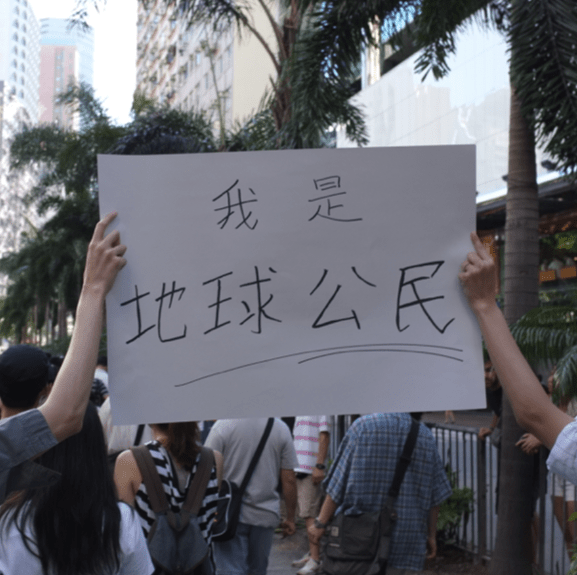
\includegraphics[width=0.7\textwidth]{c12/h-klesson1-017.png}
    \caption{「反國教」遊行標語} 
\end{figure}

反國教運動在二零一二年九月進入高峰。自九月一日開學日起,連續九天晚上有數以萬計市民在政府總部外集會抗議,學生、教師和家長絕食,「反國教」成為剛上任行政長官的梁振英的首個政治炸彈。到了九月九日,梁振英宣布取消國教科開展期,抽起「當代國情」部分,並於十月正式擱置國教科課程指引。

值得注意的是,這次運動的成功在香港的反對運動中有其獨特性。帶頭的學生組織「學民思潮」以一班中學生為核心,他們過去沒有任何政治參與的經驗,因而也沒有任何包袱和私怨,才能取得市民的同情和認可。運動本身亦容許了不同立場的抗爭者參與,無論是「愛國不愛黨」還是全面抗拒中國認同的抗爭者都可以在運動中共存。

\begin{figure}[htbp]
    \centering
    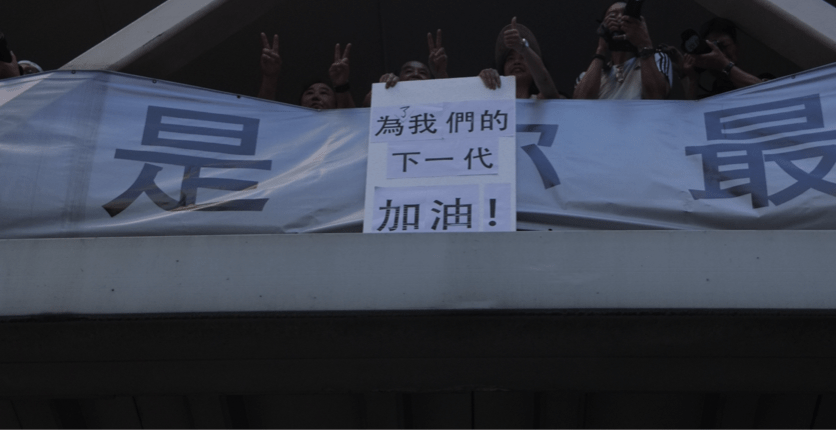
\includegraphics[width=0.7\textwidth]{c12/h-klesson1-018.png}
    \caption{「反國教」遊行標語} 
\end{figure}

雖然德育及國民教育科因為反國教運動而落幕,不過香港政府對國民教育的推動沒有停止,改為推行「沒有國民教育科的國民教育」。例如近年來中國政府和香港政府就大力資助香港學生到中國大陸交流,中國教育部提供每人每日五百五十元人民幣的補貼,香港政府又為每位香港大專生提供港幣三千元的旅費資助,使得不少交流團變相費用全免。此外,由於香港的教科書出版商大多都已被收編,與中國政府有千絲萬縷的利益關係(見\hyperref[sec:sec28]{問題二十八}),不少教科書都滲入「愛國原素」,例如加入升旗禮感受的閱讀教材等。此外,又有意見認為學校應加強中史教育來強化國家認同,但亦有歷史學者批評香港的中國歷史教育過去往往以大一統視角和漢族中心主義去書寫,既不客觀,也無助學生認清歷史。國民教育科雖然已經被抽起,但國民教育的爭議在香港仍然持續。

反國教運動顯示體制上層與社會大眾在香港身分認同的問題上嚴重脫節。國民教育遇上挫折,說到底是因為其出發點本身就是基於一系列的謬誤:先假設認識中國只有一種正確的方法,而基於這種方法自然就會得出愛國的情感;香港人只不過是因為被過去的殖民統治所蒙蔽,沒有用正確的方法認識中國,只要在教育上撥亂反正便能在認同問題上重回正軌。這假設最少有兩個問題:首先,如前文所述,香港人的中國認同一直十分豐富,對中國並非毫無認識,而認識的方法比在審查監控下的中國大陸更為多元豐富。再者,香港人過去的中國認同感並不算低,出現大幅逆轉只是近數年的事,而且集中在年輕人之間發生。他們大多都是九七後出身和成長,但他們對中國認同的抗拒程度遠高於在英治時期成長的香港人,所以「受殖民統治蒙蔽」的說法更像是為特區管治失敗找藉口。

至於為什麼香港人特別是年輕人會越來越抗拒中國認同?國民教育爭議表現出來的其實只是病徵。要尋求病因的話得從文化走進政治,看看香港特區的政治制度出了什麼問題,使得不少年輕人恨不得要和中國一刀兩斷。

\rule[-10pt]{15cm}{0.05em}

伸延閱讀:

Morris P and Vickers E (2015) Schooling, politics and the construction of identity in Hong Kong: the 2012 ‘Moral and National Education’ crisis in historical context, \textit{Comparative Education 51:3}, p305-326

曾榮光(2011):〈香港特區國民教育的議論批判〉, 《教育學報》第39卷第1-2期, p.1-24